\documentclass{article}
\usepackage[portrait, margin=1in]{geometry}
\usepackage{graphicx} 
\graphicspath{{/Users/danpost/consumer_sentiment/output/umich_figures/gaspx}{/Users/danpost/consumer_sentiment/output/umich_figures/macro_vars}}
\usepackage{amsmath}
\usepackage{hyperref}
\usepackage{threeparttable}
\usepackage{subfig}

\title{University of Michigan's Surveys of Consumers Respondents' Sensitivity to Macroeconomic Conditions}
\author{Daniel Posthumus}

\begin{document}

\maketitle

\section{Introduction}

Previous has demonstrated that Republicans and Democrats experience the economy very differently, depending on whether the White House is occupied by a President of their party or not -- previous \href{https://www.briefingbook.info/p/asymmetric-amplification-and-the}{research} by Cummings and Mahoney has shown this bias to be \textit{asymmetric}, with Republicans' partisan bias estimated to be two and a half times larger than Democrats'.

We can go beyond breaking down the top-line consumer sentiment index by partisan affiliation: the University of Michigan's Surveys of Consumers asks respondents about a host of different areas of the economy and their attitudes. The Survey only started to ask about respondents' partisan affiliation in 2017; so, starting then, we can re-create an aggregate measure of respondents' attitudes towards specific parts of the economy. Using individual-level microdata, for example, we can calculate respondents' net attitudes ((\% who have a positive attitude) - (\% who have a negative attitude) + 100) by partisan affiliation, e.g. for personal financial conditions and broad business conditions:

\centering 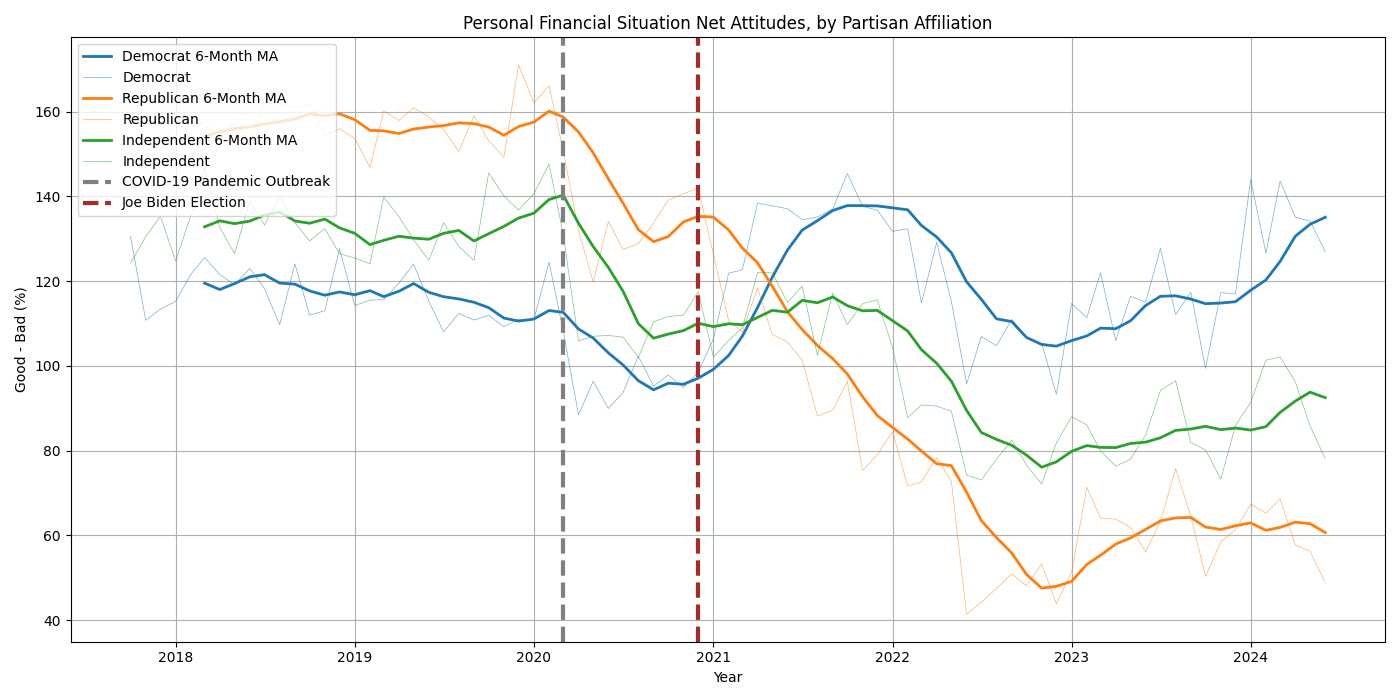
\includegraphics[width=6in]{pago_r_time_series.png} \\
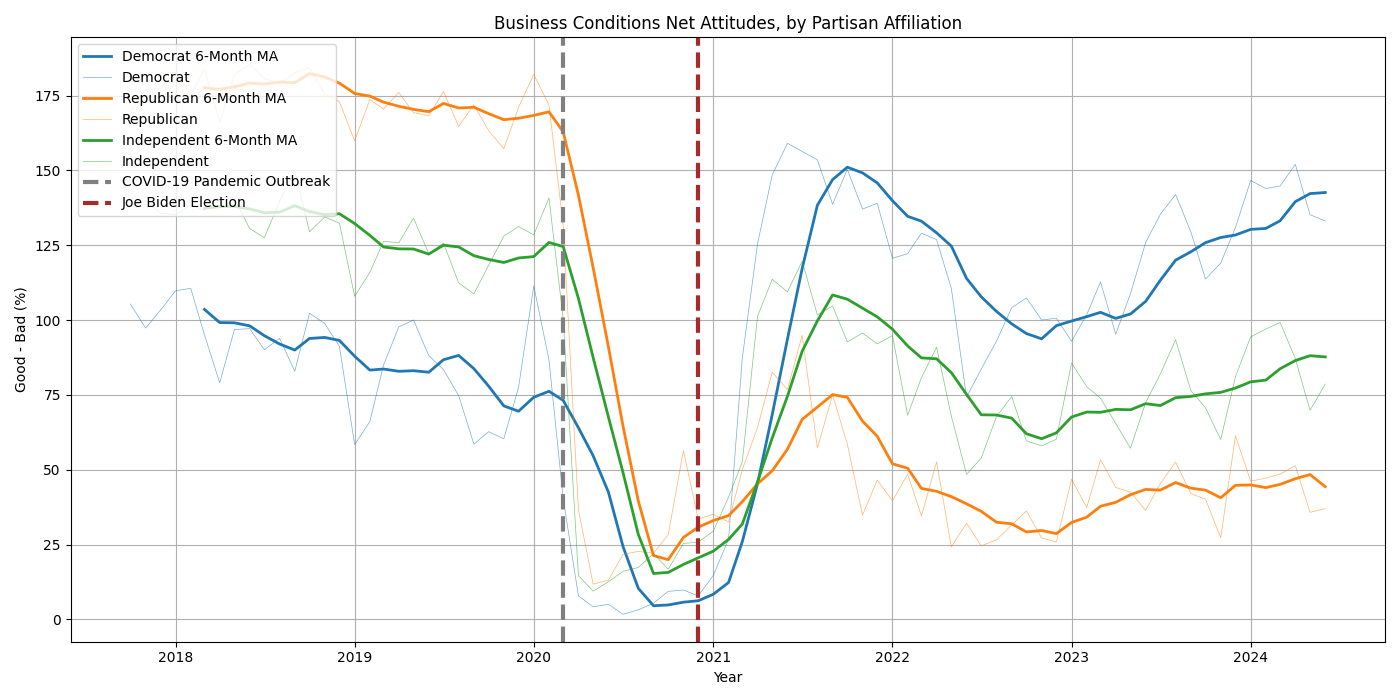
\includegraphics[width=6in]{bago_r_time_series.png}

\raggedright Using these descriptive aggregates, it's clear Republicans and Democrats experience the economy differently. In this project, we attempt to decompose those differences in attitudes towards specific parts of the economy into 1) differing pre-set biases and 2) differing sensitivity to changes in observed economic conditions. We do this through simple univariate OLS models, with standardized changes in observed economic variables as the regressors. 

\section{Gas Price Expectations}

To start with, the UMich survey asks respondents for their predicted change in gas prices over the next 1) one-year and 2) five-year periods. We can match those responses with observed gas price changes using the following model: 
\begin{gather}
	 \text{GAS\_PX\_CHG\_EXP}_{h\text{, }p\text{, }t\text{, i}} = \alpha_0 + \beta_1 Z(\text{GAS\_PX\_CHG}_t) + \epsilon_{h\text{, }p\text{, }t\text{, i}}
\end{gather}
for $h \in \{\text{1-yr, 5-yr}\}$, $p \in \{\text{Democrat, Republican, Independents}\}$, time $t$, and individual $i$. We run this model separately for whether 1) Biden was president during time $t$; 2) subsamples consisting of only Democrats, Republicans, and Independents; and 3) each horizon $h$. 

We tried several model approaches, in which the regressor varied. We tried to use 1) the level gas price, 2) the corresponding historical gas price percent change (i.e., the 1-year observed gas price change matches to the 1-year expected gas price change), and 3) the monthly gas price percent change. The monthly gas price percent change had the most robust results, although there were difficulties because there was more variance of monthly gas price changes under President Biden than President Trump. To counter this, we calculated the z-score for each month's percent change in gas prices, within the distribution of changes during 1) Trump's presidency and 2) Biden's presidency. (We follow this standardization methodology for all analysis in this project.)

We find that voters were likelier to predict higher gas price changes under President Biden, even if the percent change from the previous month was exactly average (i.e., the z-score of the change was 0). When this average gas price monthly percent change would occur, Republicans' expected 1-year gas price change would be 4.03 times higher than Democrats', and 1.5 times higher than Independents'. Republicans' expected 5-year gas price change would be 2.28 times higher than Democrats', and 1.16 times higher than Republicans'. 

\section{Zillow Home Value Index and Home-Buying Conditions} 

Unlike the gas price prediction question described above, the survey asks respondents about their attitudes towards specific parts of the economy (like home-buying conditions) by asking whether their attitudes are positive, neutral, or negative. To conduct individual-level modeling, we create a dummy variable for whether a respondent has a positive attitude towards the home-buying environment and a 0 if they have a neutral or negative attitude. Then we run the following model:
\begin{gather} 
	\text{HOM\_DUMMY}_{p,t,m,i} = \alpha_0 + \beta_1 Z(\text{ZILLOW\_INDEX\_CHG}_{t}) + \epsilon_{p,t,m}
\end{gather} 
where ZILLOW\_INDEX\_CHG is the monthly percent change in Zillow's Home Value Index, of which we take the z-score and HOM\_DUMMY is a dummy for whether individual $i$ has a positive attitude towards home-buying condition. The other variables are identical to those used in Equation (1). 

First we can see a time-series of the re-scaled regressor. \\
\centering 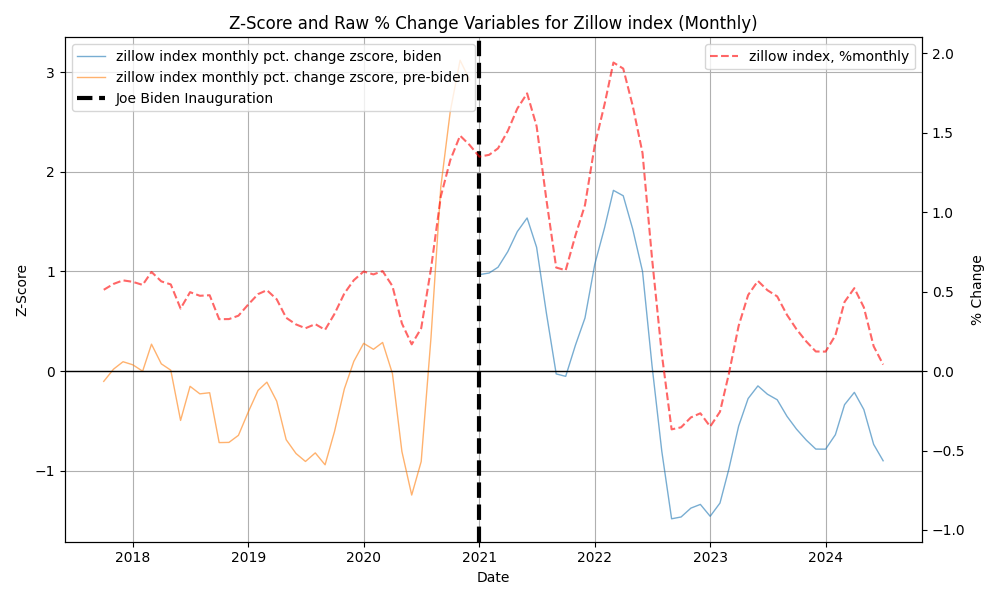
\includegraphics[width=6in]{zillow_zscore.png}

\raggedright For an mean monthly percent change in home values, Republicans were 3.09 times likelier to have positive home-buying conditions under President Trump than President Biden. That multiplier is 1.92 for Democrats and 2.43 for Independents. Critically, Republicans and Independents' $\beta_1$ is estimated to be insignificant under Biden--suggesting that for any change larger in magnitude than the mean monthly percent change, Republicans' and Independents' attitudes towards home-buying conditions wouldn't change. On the other hand, Democrats' $\beta_1$ coefficient was significant positive under Biden as well as Trump, while Republicans' and Independents' estimated $\beta_1$ coefficients were positive significant during Trump's presidency.

\section{Real Household Income}

The approach for Real Household Income was identical to Home Value: we match FRED's real household income to the University of Michigan's Surveys of Consumers re: attitudes towards whether household income will outpace inflation. Once again, we take a dummy for whether a respondent had a positive attitude and run the same regression using a standardized regressor for monthly percent change for 1) Biden's presidency and 2) Trump's presidency. 

First, none of Democrats, Republicans, nor Independents had a significant $\beta_1$ coefficient--indicating that whether they held positive attitudes towards real family incomes was set by who was President, rather than observed economic conditions. Democrats held a more positive view towards household income under Biden than Trump, while Republicans and Independents were the opposite. However, these findings match earlier work on the \textit{asymmetric} nature of partisan bias. Democrats, for a mean monthly percent change in real family income, were 1.18 times likelier to hold a positive attitude under President Biden than President Trump. Republicans, on the other hand, were 2.35 times likelier to hold a positive attitude under President Trump than President Biden, for a mean monthly percent change in real family incomes. This approximation of partisan bias is nearly twice as large for Republicans than Democrats. These coefficients are plotted below:

\centering 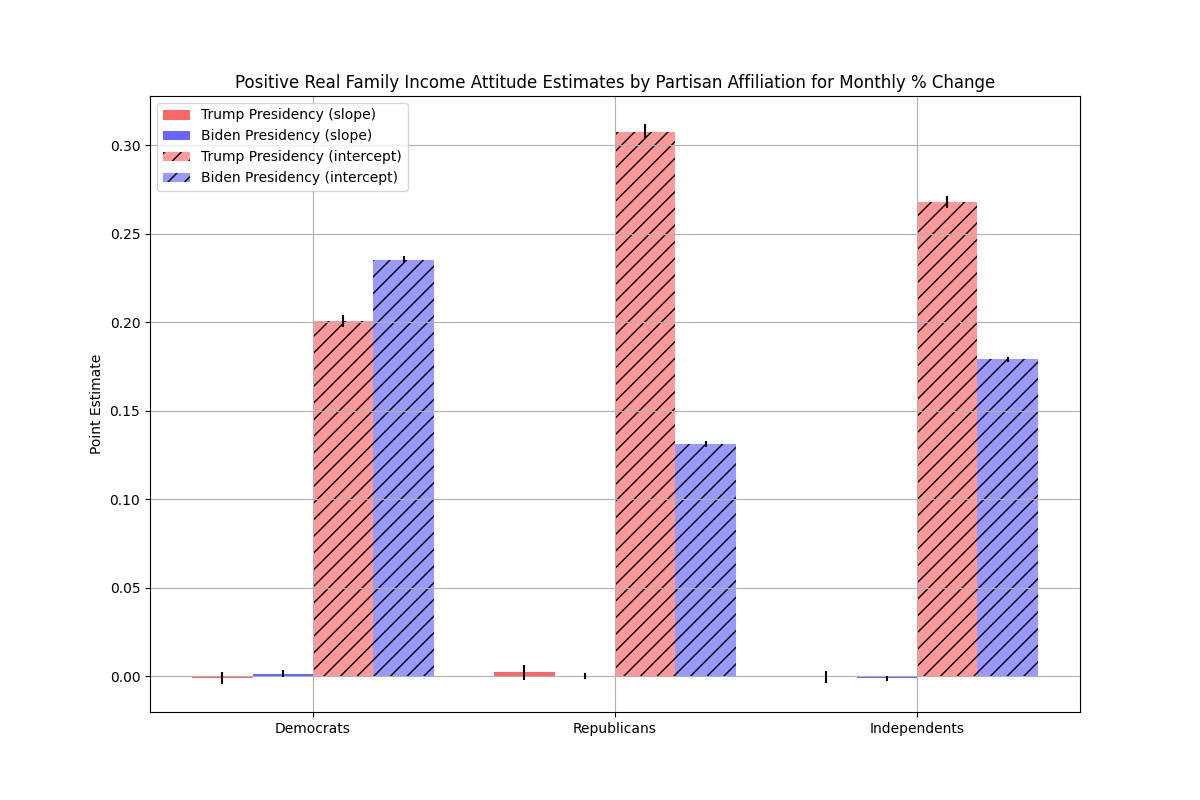
\includegraphics[width=6in]{month_rinc_party_comp_micro.png}

\raggedright \section{Used Car CPI and Car-Buying Conditions}

The approach for car-buying conditions is identical to the approaches for real household income and home-buying; here, we match a question on the survey asking after attitudes towards car-buying conditions to the BLS's Used Car CPI. Once again, during the Biden Presidency, none of Democrats, Republicans, nor Independents exhibited a significant $\beta_1$ estimated coefficient; however, each group exhibited a positive significant coefficient. Effectively, this suggests that while above-average changes in used car prices would not have affected respondents' attitudes towards car-buying conditions during Trump's presidency, they did during Biden's presidency with a positive correlation.

Then, for an average monthly percent change in used car prices, Democrats, Republicans, and Independents were likelier to have a positive attitude during the Trump presidency than Biden presidency. This gap is most magnified for Republicans; Democrats were 1.61 times likelier to have a positive attitude during Trump's presidency than Biden's, while Republicans were 2.75 times likelier. These coefficients are plotted below:

\centering 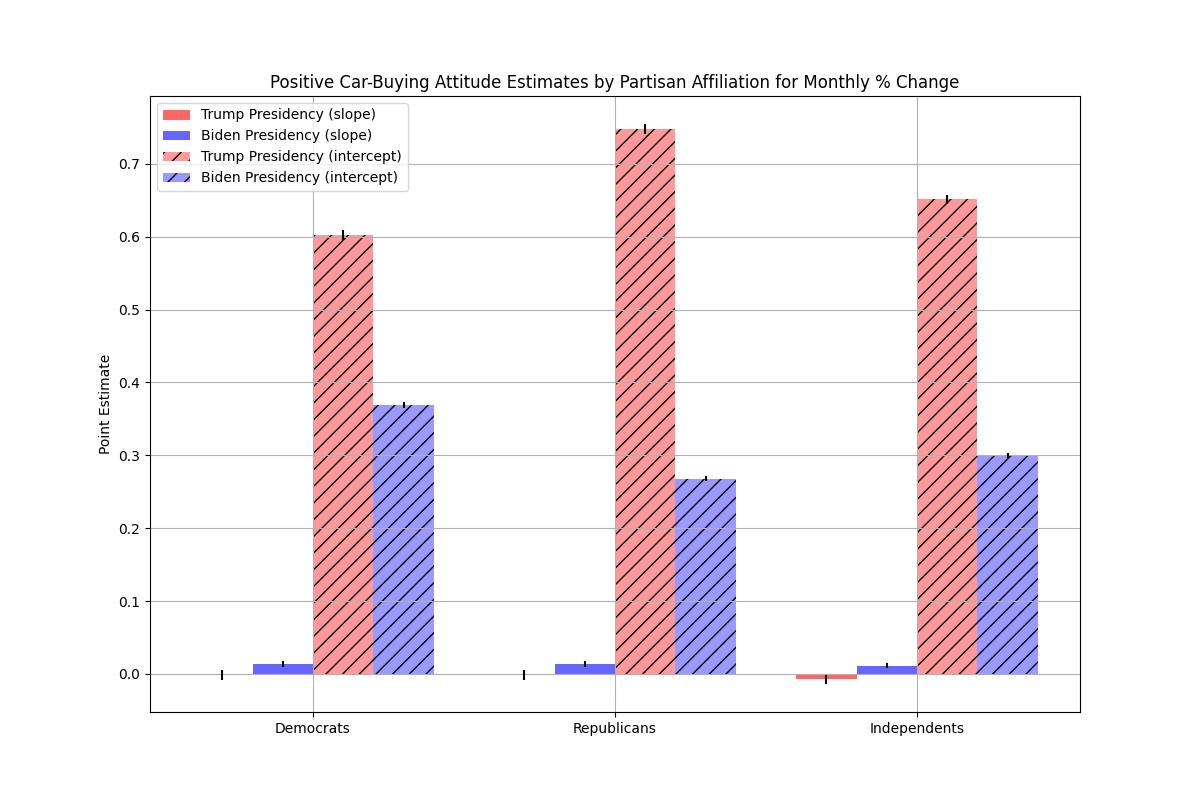
\includegraphics[width=6in]{month_car_party_comp_micro.png}

\raggedright \section{S\&P500 and Predicted Likelihood of Positive Stock Market Return}

One question on the Survey asks respondents their predicted likelihood (in percentage form) that an investment in a broad-based stock market index would yield a positive return in one year's time. Thus, for this variable there is no dummy variable creation needed; instead, we just take a respondent's predicted likelihood and use the z-score of the year-over-year percentage difference in the S\&P 500 for 1) Trump's and 2) Biden's presidency. Here we use the year-over-year percent change in the stock market because that is the exact time horizon the question is asking about--asking respondents to look one year into the future.

Interestingly, this question had the least evidence of partisan bias, as plotted below. Only Independents had a significant $\beta_1$ coefficient estimate, a positive one for during the Biden Presidency. This is also the only area where Democrats' partisan bias appears to be greater than Republicans'; for an average year-over-year percentage change in the S\&P500, Democrats appear to be 1.24 times likelier to predict a positive stock market return under Biden than Trump, while Republicans appear to be 1.05 times likelier under Trump than Biden. I suspect that this because this question is less ambiguous than those asking about attitudes towards the economy, and the prediction it is asking respondents to make is easier (since 2016, the S\&P500 has only had 2 negative return years) than asking about the expected gas price change 5 years from now. 

\centering 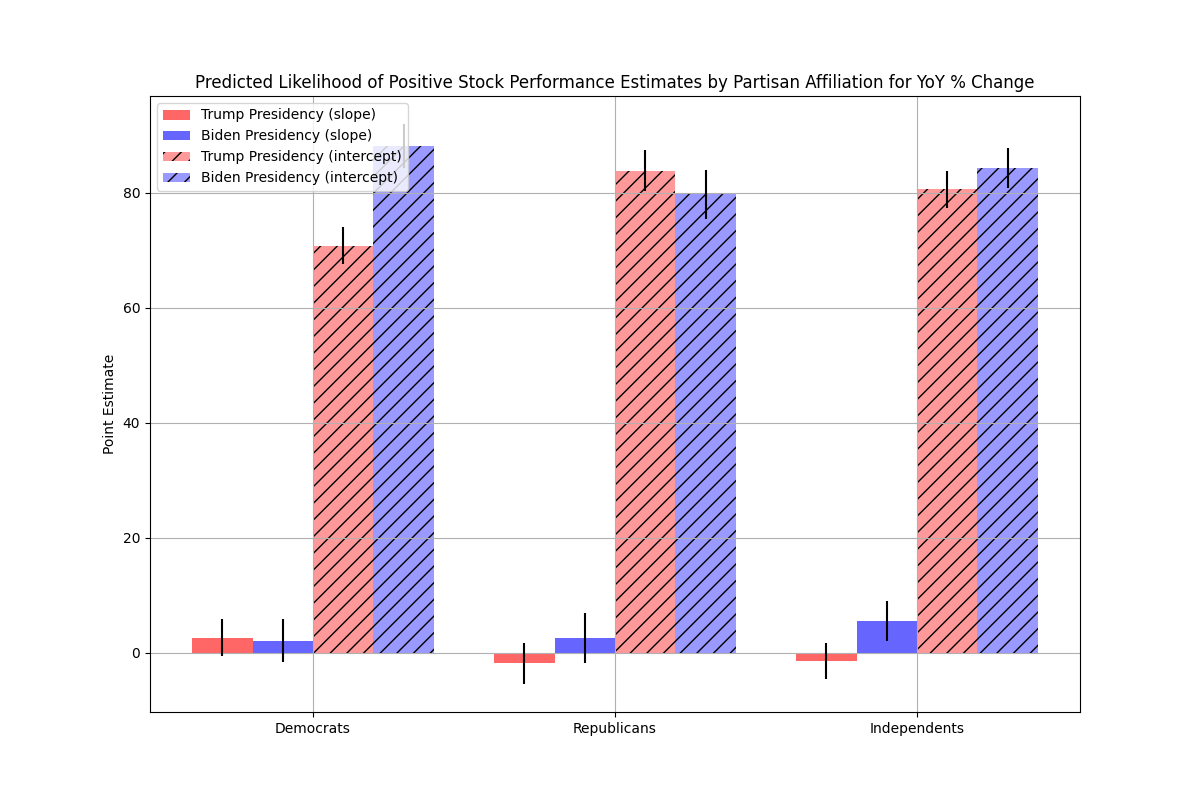
\includegraphics[width=6in]{yoy_pstk_party_comp_micro.png}

\raggedright \section{Headline CPI and Reported Unfavorable News Coverage of Inflation} 

Finally, we match changes in the US Headline CPI to respondents' reported unfavorable coverage of inflation. Two questions on the Consumer Survey ask about what economic topics respondents report having heard news coverage of. To analyze the relationship between responses to these questions and inflation, we create a dummy variable equal to 1 if a respondent answers \textit{either} of these two questions with the option of "unfavorable news coverage of rising prices". Then we used the same model as for the dummy variables described above, although here we also employ the z-score of year-over-year percent changes in headline CPI, since that is the most oft-referenced measure of inflation. First, given the large difference in variance across Trump's and Biden's presidency in headline inflation, standardizing the regressor is key as plotted below:

\centering 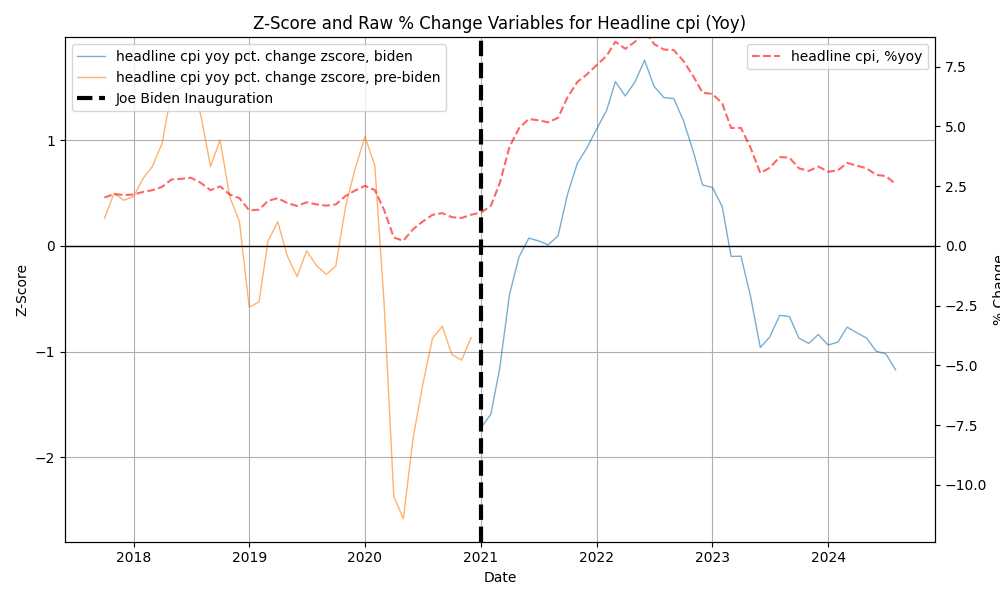
\includegraphics[width=6in]{headline_cpi_zscore.png}

\raggedright Clearly, there was a spike in inflation under President Biden that didn't occur under Trump. This is reflected in respondents' reported unfavorable news coverage of inflation -- although we can see Republicans' reported coverage happened before Independents' and Democrat's, reached a higher level, and remained elevated longer. 

\centering 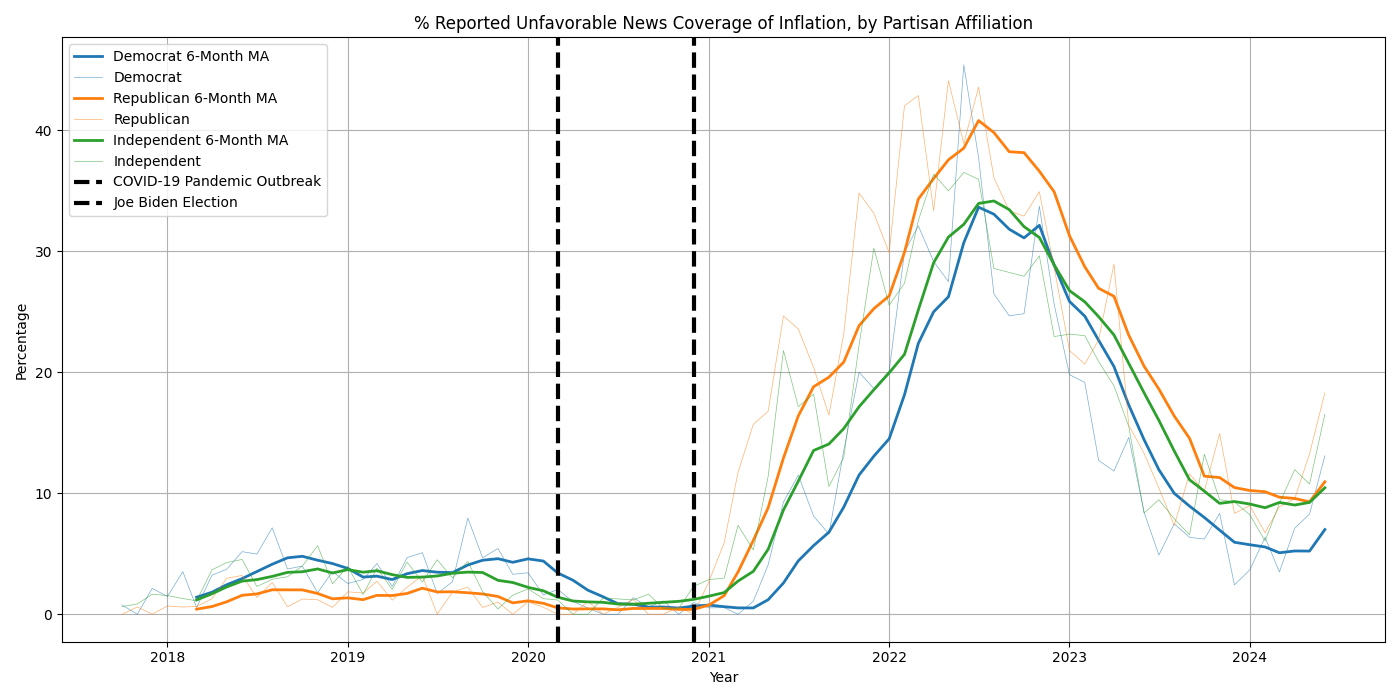
\includegraphics[width=6in]{newsrn_u_pri_time_series.png}

\raggedright Unsurprisingly, there is a significant positive $\beta_1$ coefficient for Democrats, Republicans, and Independents during either the Trump or Biden presidency. The gap seen above appears to be driven by pre-set bias ($\alpha_0$), rather than heightened sensitivity to increasing inflation. For an average change in year-over-year inflation, Republicans were 20.07 times likelier to report unfavorable news coverage of inflation under Biden than Trump, while that figure is 5.46 times for Democrats and 7.82 for Independents. Those coefficients are plotted below:

\centering 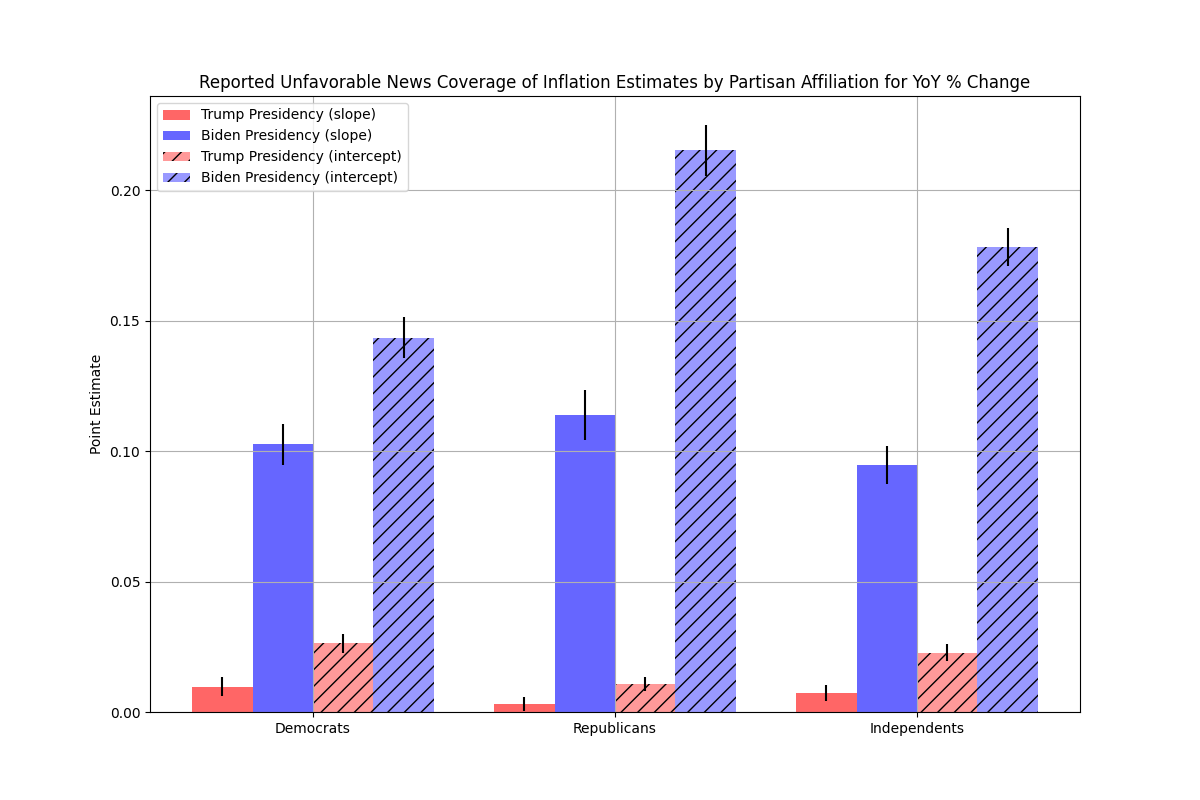
\includegraphics[width=6in]{yoy_news_pri_party_comp_micro.png}

\end{document}